\documentclass[letterpaper]{article}
\usepackage{natbib}
\usepackage[utf8]{inputenc}
\usepackage{graphicx}
\usepackage{color}
\usepackage{multirow}
\usepackage{amsmath}
\usepackage{array}
\usepackage{subcaption}
\usepackage{mathpazo}
\usepackage{listings}
\usepackage[a4paper]{geometry}
\usepackage{float}

\definecolor{pblue}{rgb}{0.13,0.13,1}
\definecolor{pgreen}{rgb}{0,0.5,0}
\definecolor{pred}{rgb}{0.9,0,0}
\definecolor{pgrey}{rgb}{0.46,0.45,0.48}


\title{Data structures and Algorithms (INFO-F413) \\
\Large  Assignment 1: Binary Space Partitions}
\author{\Large Hakim Boulahya \\
hboulahy@ulb.ac.be\\
\\
Université Libre de Bruxelles
}




\begin{document}


\lstset{language=Python,
  showspaces=false,
  showtabs=true,
  breaklines=true,
  showstringspaces=false,
  breakatwhitespace=true,
  commentstyle=\color{pgreen},
  keywordstyle=\color{pblue},
  stringstyle=\color{pred},
  basicstyle=\footnotesize,
  numbers=left,
  moredelim=[il][\textcolor{pgrey}]{$ $},
  moredelim=[is][\textcolor{pgrey}]{\%\%}{\%\%}
}


\maketitle
\tableofcontents
\newpage

\section{Implementation}


\subsection{Solution for the subproblems}

\subsubsection{Intersection}

\paragraph{}

To find the intersection point between the line that is going through a segment
and another segment we resolve a system of equations of the two linear equations
representing the line of the segments. Let $a_1x + b_1y + c_1$ and
$a_2x + b_2y + c_2$ two lines, we know that the intersection point of the two lines,
if it exists, is a point that is on both lines i.e. the results of the following system:
\begin{equation}
  \label{eq:lin_sys}
\begin{cases}
a_1x + b_1y + c_1 = 0 \\
a_2x + b_2y + c_2 = 0
\end{cases}
\end{equation}

Because we represent a segment with two coordinates $(x_1, y_1)$ and $(x_2, y_2)$,
we have to find the equation of the line going through a segment using those
coordinates to get the intersection point.
We will base our solution on the point-slope formula:

\paragraph{Slope}
Let $(x_1, y_1)$ and $(x_2, y_2)$ the pair of coordinates corresponding to a segment,
the slope of this segment is the value $m$ such as:

\begin{equation}
m = \frac{y_2 - y_1}{x_2 - x_1}
\end{equation}

By using one point on the line, i.e. a segment coordinate,
 and replacing the second point of the point-slope formula by the variables
 $(x, y)$ we can deduce the coefficients of the line equation as follow:


\begin{equation}
 m = \frac{y - y_1}{x - x_1} \iff
-mx + y + (mx_1 - y_1) = 0
\end{equation}

We can now get the intersection point of a line going through a segment and another
segment by using the results explained above. First we calculate slopes
of both segments, says $m_1$ and $m_2$. If $m_1 =m_2$ the segments have the same
slopes therefore they are parallele meaning that there is no intersection.
If the slopes are different, we get the intersection of the two lines going through
both segments by solving the system of equations in (\ref{eq:lin_sys}).
Because we need the intersection of a line and a segment and not two lines, we
have to verify that the second segment is indeed cut by the line of the first segment.
For this we use the outer product, described in the next section,
to check if the coordinates of the second segment are on different side of the line.
If coordinates of the second segment are on different sides, in means that the line
cuts off the segment.

\subsubsection{Split space}

\paragraph{}

For checking on which side of a line a segment is, we use the outer product between
the line and both point of the segment that we want to check. To check if
the side of a point $(x, y)$ regarding a line that is going through a segment
$(x_1, y_1)$, $(x_2, y_2)$ we first evaluate the outer product $d$:

$$
d = (x - x_1)(y_2 - y_1) - (y - y_1)(x_2 - x_1)
$$


if $d > 0$ the point is on one side, otherwise it is on the other side.
With this formula, we can define the side of a segment by checking if both
coordinates are one the same side side. If both coordinates are one different sides it means
that the line cuts the segment.


\subsection{Inputs}

For this experiment we propose three methods of inputs generation:

\begin{itemize}
  \item Completely random inputs. No pattern will be followed when generating those inputs,
  and both coordinates of all segments will be completely random.
  \item Inputs following a \textit{triangle}-like pattern, meaning that each pattern
  will be composed of two side of a triangle, without the base.
  \item Inputs with all sides of a \textit{triangle}-like pattern.
\end{itemize}

\begin{figure}[H]
    \begin{subfigure}{.5\textwidth}
      \centering
      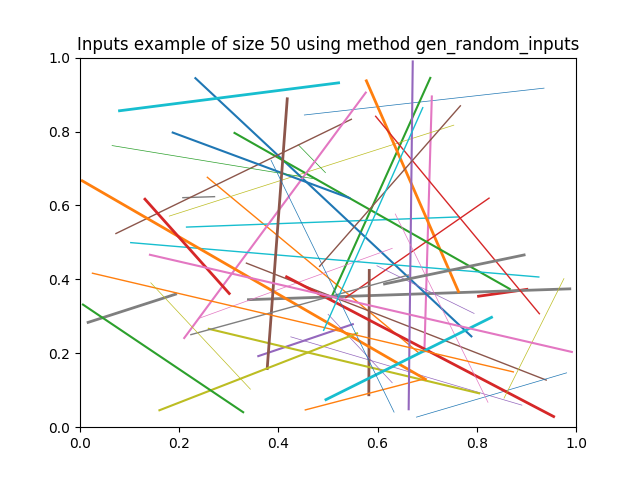
\includegraphics[width=1\linewidth]{images/assign1/gen_inputs_random}
      \caption{Completely random inputs}
      \label{fig:random_inputs}
    \end{subfigure}
    \begin{subfigure}{.5\textwidth}
      \centering
      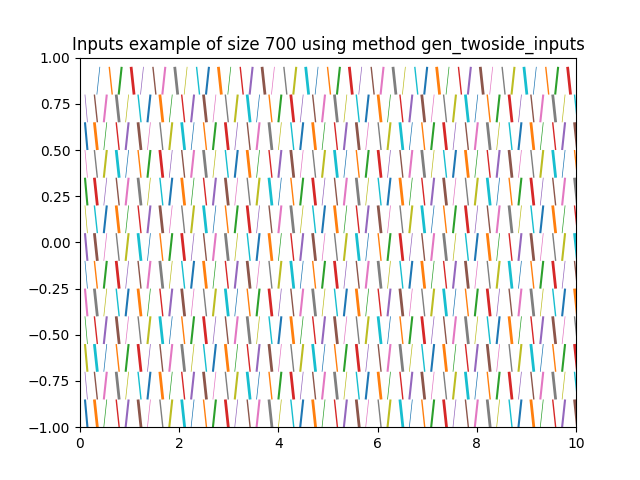
\includegraphics[width=1\linewidth]{images/assign1/gen_inputs_triangle}
      \caption{Inputs following a \textit{triangle} pattern with two segments (without the base).}
      \label{fig:triangle_inputs}
    \end{subfigure}
    \begin{subfigure}{.5\textwidth}
      \centering
      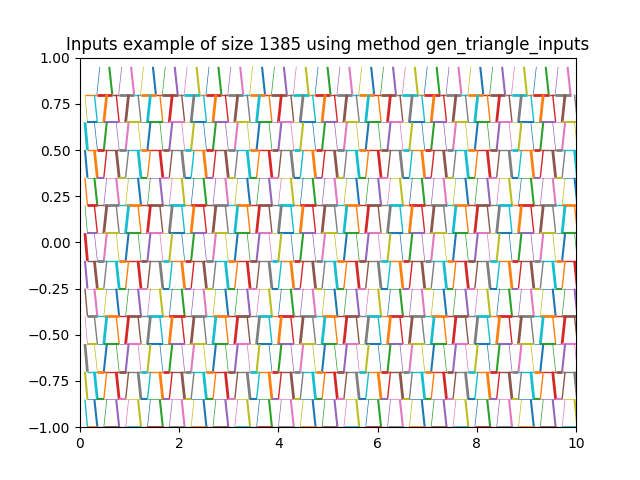
\includegraphics[width=1\linewidth]{images/assign1/gen_inputs_fulltriangle}
      \caption{Inputs following a \textit{triangle} pattern with three segments (with the base).}
      \label{fig:full_triangle_inputs}
    \end{subfigure}
    \caption{Type of generated inputs}
    \label{fig:inputs}
\end{figure}

\subsection{Algorithm}

To get the size of the binary partition size, we implemented the algorithm as described
in the assignment description, using the methods describe above for the inputs and
the subproblems:

\begin{itemize}
  \item Generate a list of segments
  \item Shuffle this list
  \item Take first element and split in two sides
  \item Run recursively the algorithm on both sides
\end{itemize}


\section{Results}

\paragraph{}

This section shows figures of results of the above algorithms. Each figure
contains different plots showing the binary space size (red dots) for a given
size and input generation method. The upper bound is shown in a blue line.

\begin{figure}[H]
    \begin{subfigure}{.33\textwidth}
      \centering
      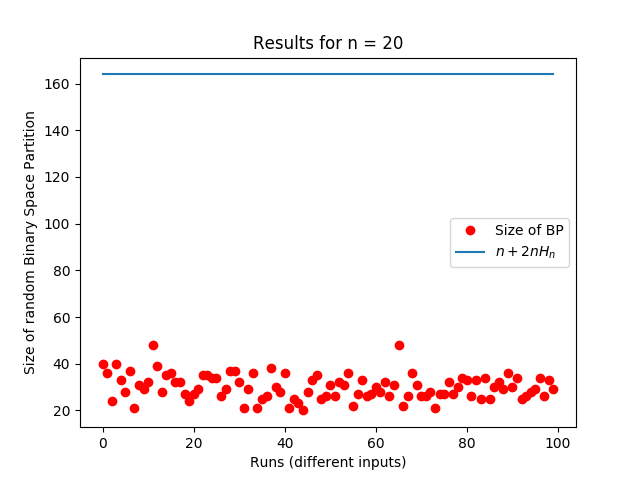
\includegraphics[width=1\linewidth]{images/assign1/random/inputs_20}
      \caption{$n = 20$}
    \end{subfigure}
    \begin{subfigure}{.33\textwidth}
      \centering
      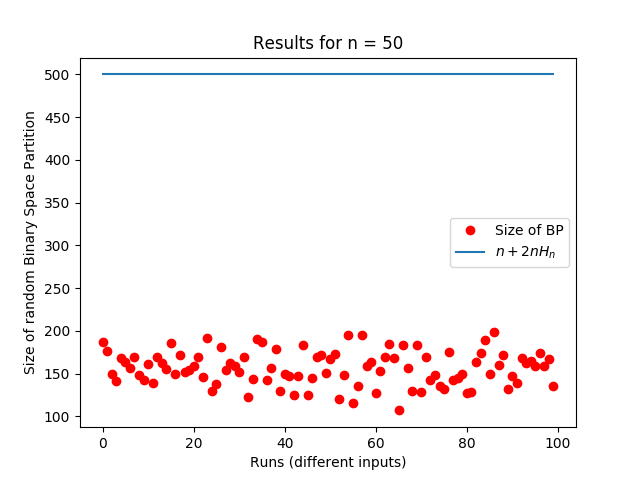
\includegraphics[width=1\linewidth]{images/assign1/random/inputs_50}
      \caption{$n = 50$}
    \end{subfigure}
    \begin{subfigure}{.33\textwidth}
      \centering
      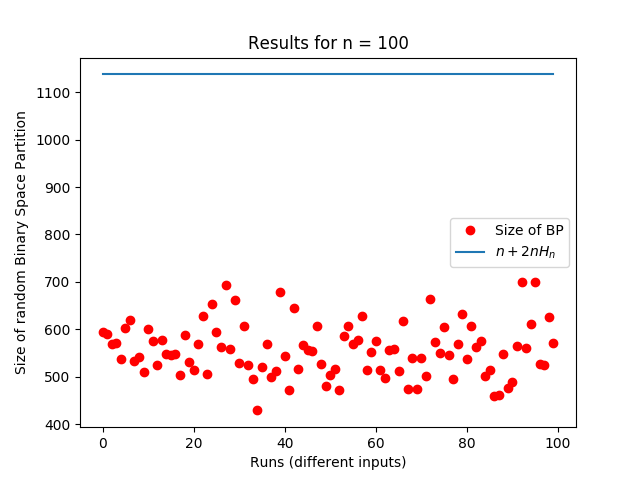
\includegraphics[width=1\linewidth]{images/assign1/random/inputs_100}
      \caption{$n = 100$}
    \end{subfigure}
    \begin{subfigure}{.33\textwidth}
      \centering
      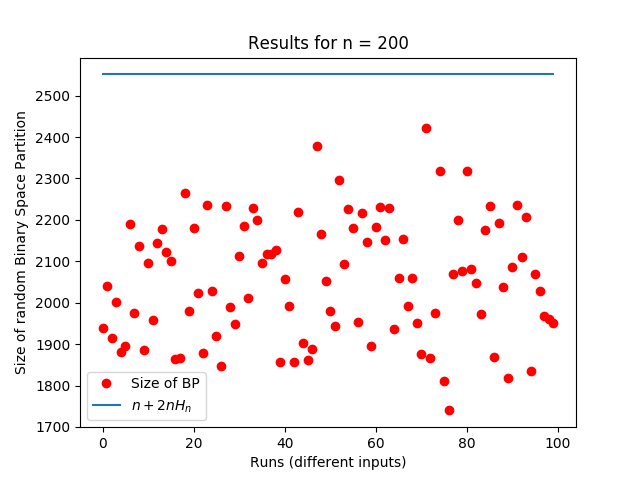
\includegraphics[width=1\linewidth]{images/assign1/random/inputs_200}
      \caption{$n = 200$}
    \end{subfigure}
    \begin{subfigure}{.33\textwidth}
      \centering
      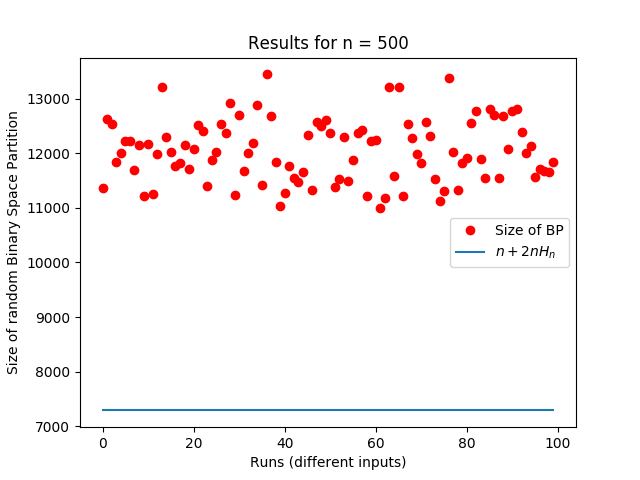
\includegraphics[width=1\linewidth]{images/assign1/random/inputs_500}
      \caption{$n = 500$}
    \end{subfigure}
    \begin{subfigure}{.33\textwidth}
      \centering
      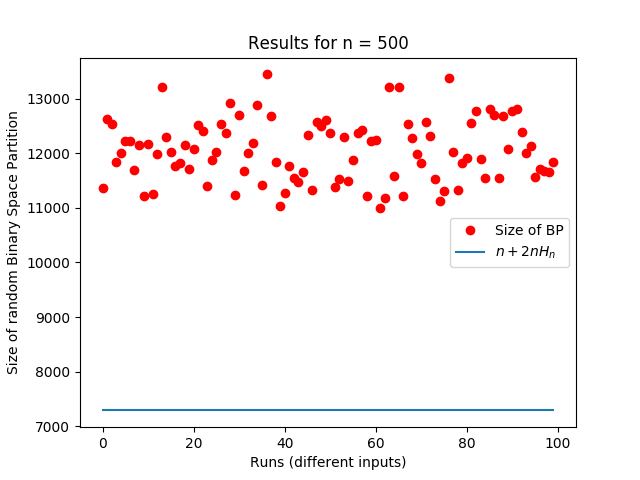
\includegraphics[width=1\linewidth]{images/assign1/random/inputs_500}
      \caption{$n = 700$}
    \end{subfigure}
    \caption{Visualization of a the binary space partition size using
    random inputs as shown in Figure \ref{fig:random_inputs}.
    Those plots show results for
    different values of n with 100 expirements per value. Red points represent
    the BP size and the blue line the upper bound $n + 2nH_n$.}
    \label{fig:expirements_random}
\end{figure}

\begin{figure}[H]
    \begin{subfigure}{.33\textwidth}
      \centering
      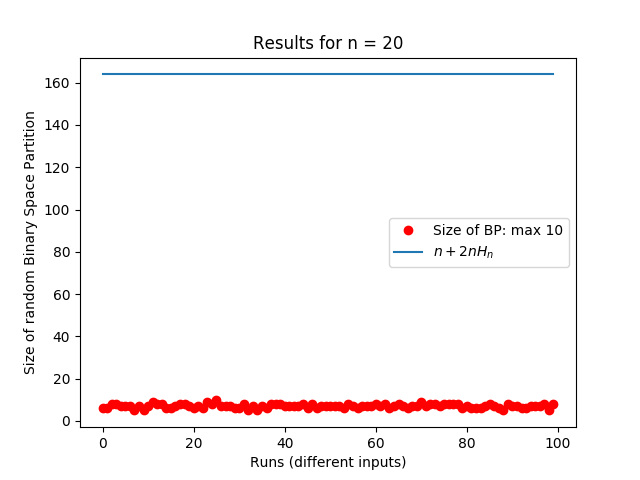
\includegraphics[width=1\linewidth]{images/assign1/triangle/inputs_20}
      \caption{$n = 20$}
    \end{subfigure}
    \begin{subfigure}{.33\textwidth}
      \centering
      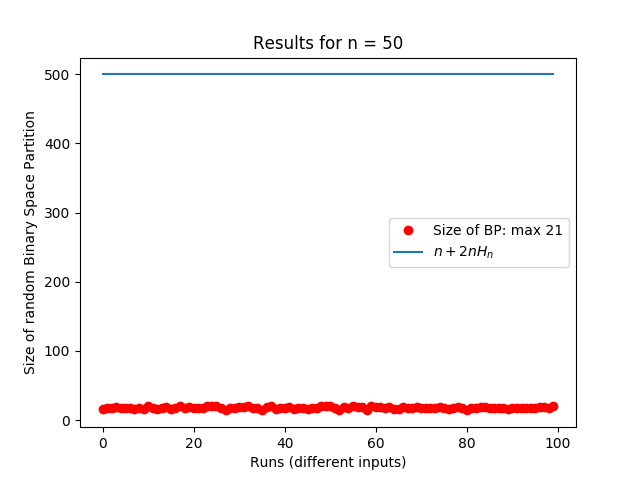
\includegraphics[width=1\linewidth]{images/assign1/triangle/inputs_50}
      \caption{$n = 50$}
    \end{subfigure}
    \begin{subfigure}{.33\textwidth}
      \centering
      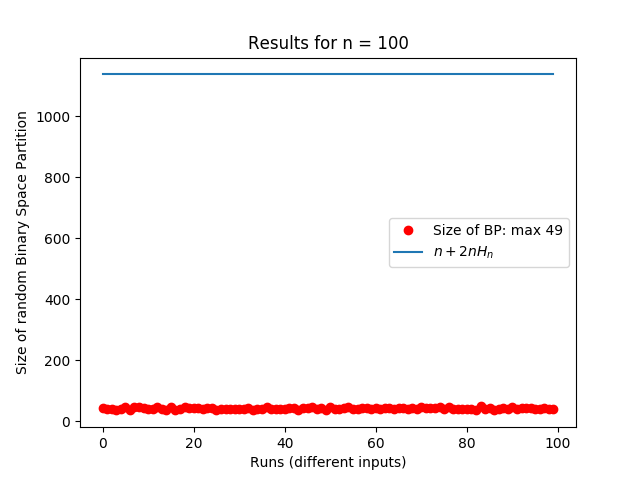
\includegraphics[width=1\linewidth]{images/assign1/triangle/inputs_100}
      \caption{$n = 100$}
    \end{subfigure}
    \begin{subfigure}{.33\textwidth}
      \centering
      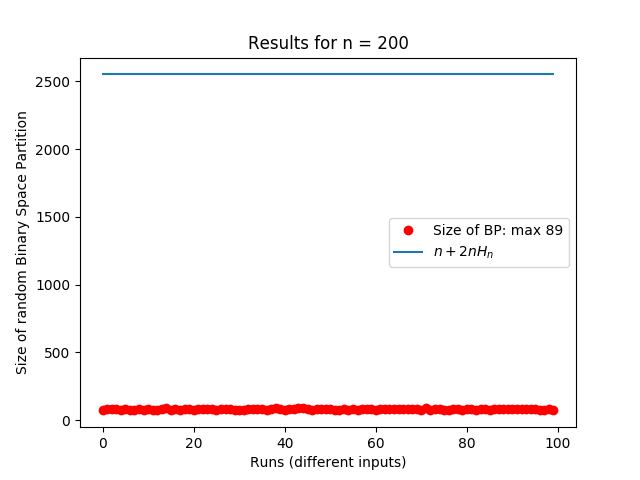
\includegraphics[width=1\linewidth]{images/assign1/triangle/inputs_200}
      \caption{$n = 200$}
    \end{subfigure}
    \begin{subfigure}{.33\textwidth}
      \centering
      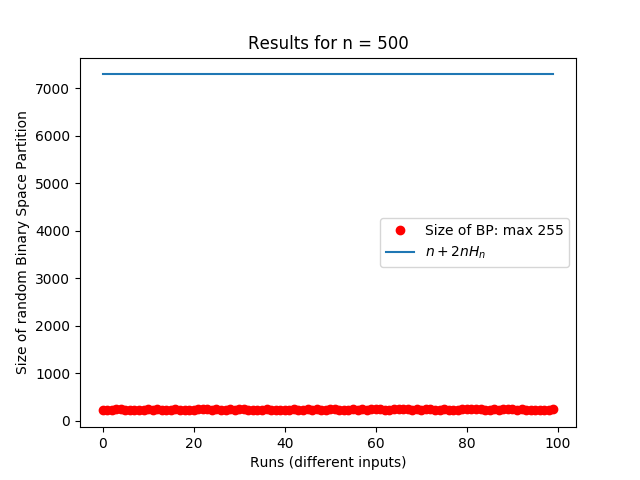
\includegraphics[width=1\linewidth]{images/assign1/triangle/inputs_500}
      \caption{$n = 500$}
    \end{subfigure}
    \begin{subfigure}{.33\textwidth}
      \centering
      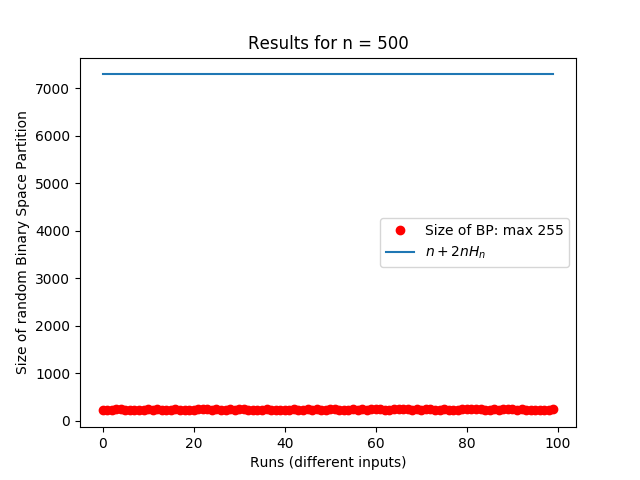
\includegraphics[width=1\linewidth]{images/assign1/triangle/inputs_500}
      \caption{$n = 700$}
    \end{subfigure}
    \caption{Visualization of a the binary space partition size using
    second method of inputs generation as shown in Figure \ref{fig:triangle_inputs}.
    Those plots show results for
    different values of n with 100 expirements per value. Red points represent
    the BP size and the blue line the upper bound $n + 2nH_n$.}
    \label{fig:expirements_triangle}
\end{figure}

\begin{figure}[H]
    \begin{subfigure}{.33\textwidth}
      \centering
      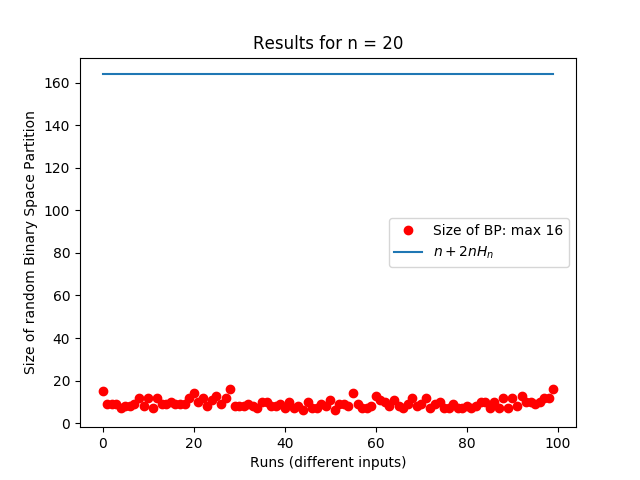
\includegraphics[width=1\linewidth]{images/assign1/fulltriangle/inputs_20}
      \caption{$n = 20$}
    \end{subfigure}
    \begin{subfigure}{.33\textwidth}
      \centering
      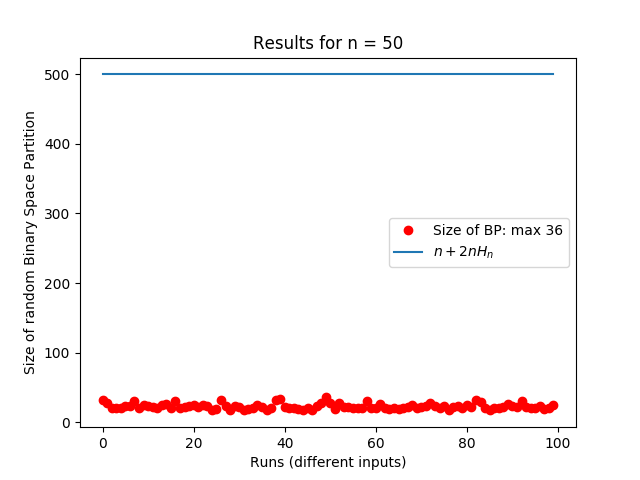
\includegraphics[width=1\linewidth]{images/assign1/fulltriangle/inputs_50}
      \caption{$n = 50$}
    \end{subfigure}
    \begin{subfigure}{.33\textwidth}
      \centering
      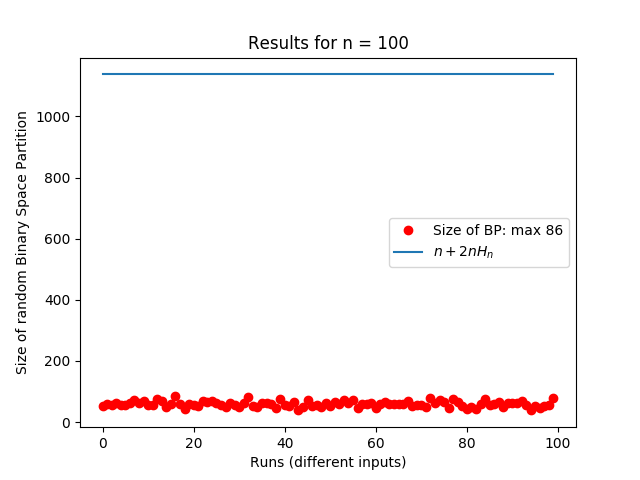
\includegraphics[width=1\linewidth]{images/assign1/fulltriangle/inputs_100}
      \caption{$n = 100$}
    \end{subfigure}
    \begin{subfigure}{.33\textwidth}
      \centering
      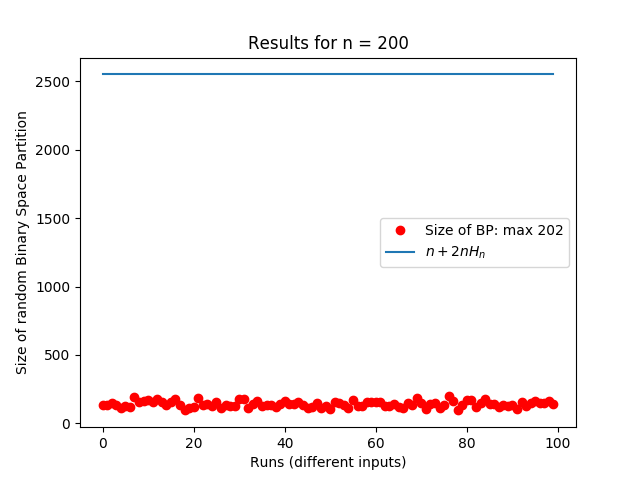
\includegraphics[width=1\linewidth]{images/assign1/fulltriangle/inputs_200}
      \caption{$n = 200$}
    \end{subfigure}
    \begin{subfigure}{.33\textwidth}
      \centering
      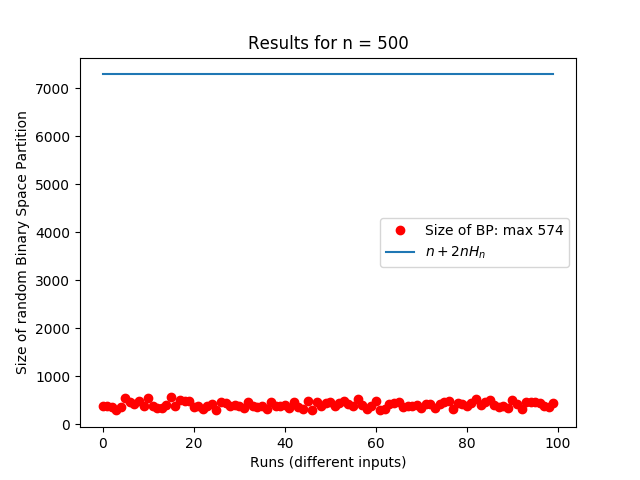
\includegraphics[width=1\linewidth]{images/assign1/fulltriangle/inputs_500}
      \caption{$n = 500$}
    \end{subfigure}
    \begin{subfigure}{.33\textwidth}
      \centering
      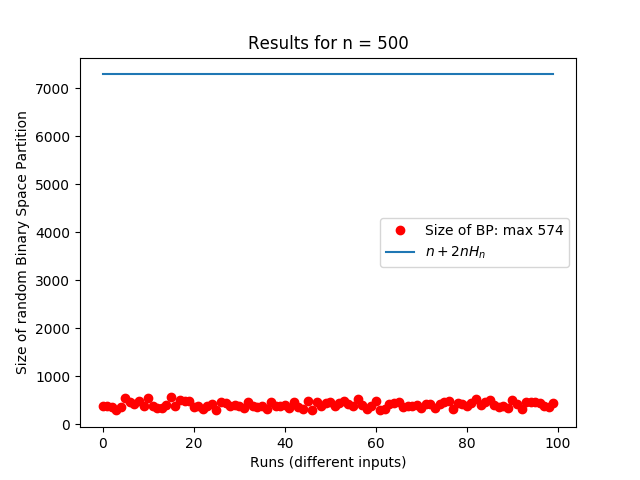
\includegraphics[width=1\linewidth]{images/assign1/fulltriangle/inputs_500}
      \caption{$n = 700$}
    \end{subfigure}
    \caption{Visualization of a the binary space partition size using
    third method of inputs generation as shown in Figure \ref{fig:full_triangle_inputs}.
    Those plots show results for
    different values of n with 100 expirements per value. Red points represent
    the BP size and the blue line the upper bound $n + 2nH_n$.}
    \label{fig:expirements_fulltriangle}
\end{figure}

\subsection{Discussion}

\paragraph{}


From the results presented above, the main analysis that we can make is that
the generation method of the inputs have a big impact on the binary space size.
We expected the random method to not respect the upper bound due to the fact
that it does not follow the definition of the problem given in the book:
segments must not intersect. With these inputs, we found that for a large n,
the binary space size always go beyond the upper bound.

\paragraph{}

With the generation of inputs that follows
a pattern and do not intersect,
the results show that the binary space size is always below the upper bound.
Indeed with the two methods for input generation that we used, the upper bound is
always respected. The main difference between the method with 3 segments
per pattern is that
the binary space size increase compare to the pattern with only 2 segments.

\paragraph{}

We conclude from these results that the inputs generation is important.
The layout of the segments on the plance seems to give a higher binary space size
for the same number of inputs and without
going beyond the upper bound. We suppose that random generated inputs will also
follow this behaviour, based on the results, if the non-intersecting segments
condition is respected. Random non-intersection segements have not been implemented and
it might be interesting to find a way to generate non-intersecting segments to confirm
these results.

\newpage

\section{Source Code}

\subsection{Description}

\paragraph{}

The binary space partition algorithm is implemented in the \texttt{bin\_space} function.
Generation of inputs is made in functions named \texttt{gen\_<method>\_inputs}.
The \texttt{main} function can be configured to run multiple experiments (\texttt{nepoch})
for different n (\texttt{nvalues}) using a defined inputs generation method.


\subsection{Python script}


\begin{lstlisting}
#!/usr/bin/python3

import logging
import os
import sys
from datetime import datetime
from fractions import Fraction
from random import shuffle

import matplotlib.pyplot as plt
import numpy as np
from matplotlib import colors as mcolors
from matplotlib.collections import LineCollection

logging.basicConfig(level=logging.ERROR)

# Specify backend, to allow usage from terminal
plt.switch_backend('agg')


def get_slope(point0, point1):
    x1, y1 = point0
    x2, y2 = point1
    return np.divide(y2 - y1, x2 - x1)

def lin_eq(line):
    x1, y1 = line[0]
    m = get_slope(*line)
    return -m, 1, np.dot(m, x1) - y1

def intersect_point(line0, line1):
    s0, s1 = get_slope(*line0), get_slope(*line1)
    if s0 == s1:
        raise ValueError("line0: %s and line1: %s have the same slope." % (line0, line1))
    a0, b0, c0 = lin_eq(line0)
    a1, b1, c1 = lin_eq(line1)
    a = np.array(((a0, b0), (a1, b1)))
    b = np.array((-c0, -c1))
    return np.linalg.solve(a, b)

def outer_product(el, coord):
    (x1, y1), (x2, y2) = el[0], el[1]
    x, y = coord
    d = np.subtract(np.dot(x - x1, y2 - y1), np.dot(y - y1, x2 - x1))
    return d

def in_first_side(el, coord):
    return outer_product(el, coord) >= 0


def in_second_side(el, coord):
    return outer_product(el, coord) < 0

def split_space(el, elements):
    side0, side1 = [], []
    for element in elements:
        coord0, coord1 = element
        if in_first_side(el, coord0) and in_first_side(el, coord1):
            side0.append(element)
        elif in_second_side(el, coord0) and in_second_side(el, coord1):
            side1.append(element)
        elif in_first_side(el, coord0):
            intersect = intersect_point(el, element)
            side0.append((coord0, intersect))
            side1.append((intersect, coord1))
        else:
            intersect = intersect_point(el, element)
            side0.append((coord1, intersect))
            side1.append((intersect, coord0))
    return side0, side1

def _bin_space(elements):
    logging.debug('_bin_space on %s', elements)
    if len(elements) < 2:
        return len(elements)
    else:
        el = elements[0]
        elements = elements[1:]
        side0, side1 = split_space(el, elements)
        logging.debug('Split sides: %s --- %s', side0, side1)
        return _bin_space(side0) + _bin_space(side1)

def bin_space(elements):
    shuffle(elements)
    return _bin_space(elements)

def gen_random_inputs(n, seed=None):
    inputs = []
    if seed is not None:
        np.random.seed(seed)
    for i in range(n):
        coord0, coord1 = np.random.rand(2), np.random.rand(2)
        inp = (coord0, coord1)
        inputs.append(inp)
    return inputs

def gen_triangle_inputs(n):
    inputs = []
    coord0, coord1 = np.array([0.1, 0.8]), np.array([0.15, 0.95])
    big_lag, small_lag = 0.09, 0.15
    lag = 0.1
    for i in range(n):
        previous_coord0, previous_coord1 = coord0, coord1
        lag0, lag1 = (big_lag + lag, small_lag + lag) if i % 2 == 0 else (small_lag + lag, big_lag + lag)
        coord0, coord1 = np.array([coord1[0] + lag0, coord0[1]]), np.array([coord1[0] + lag1, coord1[1]])
        inp = (coord0, coord1)
        inputs.append(inp)
        new_line = coord1[0] > 10
        if new_line:
            coord0[1] -= 0.15
            coord1[1] -= 0.15
            coord0[0] = 0.15
            coord1[0] = 0.1
        else:
            inputs.append((previous_coord0, coord0))
    return inputs

def gen_twoside_inputs(n):
    inputs = []
    coord0, coord1 = np.array([0.1, 0.8]), np.array([0.15, 0.95])
    big_lag, small_lag = 0.09, 0.15
    lag = 0.1
    new_line = False
    for i in range(n):
        previous_coord0, previous_coord1 = coord0, coord1
        lag0, lag1 = (big_lag + lag, small_lag + lag) if i % 2 == 0 else (small_lag + lag, big_lag + lag)
        coord0, coord1 = np.array([coord1[0] + lag0, coord0[1]]), np.array([coord1[0] + lag1, coord1[1]])
        inp = (coord0, coord1)
        inputs.append(inp)
        new_line = coord1[0] > 10
        if new_line:
            coord0[1] -= 0.15
            coord1[1] -= 0.15
            coord0[0] = 0.15
            coord1[0] = 0.1
    return inputs

def show_inputs(inputs, results_dir, method_name):
    colors = [mcolors.to_rgba(c)
              for c in plt.rcParams['axes.prop_cycle'].by_key()['color']]
    line_segments = LineCollection(inputs, linewidths=(0.5, 1, 1.5, 2),
                                   colors=colors, linestyle='solid')
    fig, ax = plt.subplots()
    ax.set_xlim(0, 1)
    ax.set_ylim(0, 1)
    ax.add_collection(line_segments)
    ax.set_title('Inputs example of size %s using method %s' % (len(inputs), method_name))
    fig.savefig(os.path.join(results_dir, 'inputs_sample_%s.png' % len(inputs)))

def show_result(n, results, nepoch, results_dir):
    fig = plt.figure()
    plt.plot(np.arange(nepoch), results, 'ro')
    plt.plot(np.arange(nepoch), np.full(nepoch, expected_size(n)))
    plt.title('Results for n = %s' % n)
    plt.xlabel('Runs (different inputs)')
    plt.ylabel('Size of random Binary Space Partition')
    plt.legend(['Size of BP: max %s' % max(results), r'$n + 2nH_n$'])
    f = os.path.join(results_dir, 'inputs_%s' % n)
    if os.path.exists(f + '.png'):
        i = 0
        init_f = f
        f = init_f + '_' + str(i)
        while os.path.exists(f + '.png'):
            i += 1
            f = init_f + '_' + str(i)
    fig.savefig(f + '.png')

def expected_size(n):
    return np.add(n, 2 * np.dot(n, H(n)))

def H(n):
    return sum(Fraction(1, d) for d in range(1, n + 1))

def main():
    results_dir = os.path.join('results', str(datetime.now()))
    os.makedirs(results_dir, exist_ok=True)
    nepoch = 100
    nvalues = [2, 10, 20, 50, 100, 200, 500]
    sizes = {}
    inputs_func = gen_random_inputs
    print('Input method: %s' % inputs_func.__name__)
    for n in nvalues:
        sizes[n] = []
        print('Running for n=%s' % n)
        inputs = inputs_func(n)
        show_inputs(inputs, results_dir, inputs_func.__name__)
        for epoch in range(nepoch):
            print(epoch, end=', ')
            sys.stdout.flush()
            inputs = inputs_func(n)
            sizes[n].append(bin_space(inputs))
        print()
        print(sizes)
        show_result(n, sizes[n], nepoch, results_dir)

if __name__ == "__main__":
    main()

\end{lstlisting}

\section*{References}

\paragraph{Outer product} https://math.stackexchange.com/questions/274712/calculate-on-which-side-of-a-straight-line-is-a-given-point-located
\paragraph{Intersection} http://infohost.nmt.edu/tcc/help/lang/python/examples/homcoord/Line-intersect.html
\paragraph{Harmonic Series heuristic} https://stackoverflow.com/questions/404346/python-program-to-calculate-harmonic-series\#404425




\end{document}
